For our implementation we used the commercially available software Tableau Desktop provided by Tableau\textregistered. The interaction with Tableau Desktop works by translating drag-and-drop actions into data queries via an intuitive user interface. For a first introduction of the user interface see also Ko and Chang~\cite{Ko.2017}. 
Tableau can be connected to multiple data sources like spreadsheets or text files, or for instance to a big data, relational database on a server and others. Here we used the provided 26 comma-separated values (CSV) files and build the corresponding data model based on the information about the MIMIC-III data structure provided by the PhysioNet website (https://mimic.physionet.org/). Fig.~\ref{f1} shows an overview of the used data model to interact with the data. We planed to use a patient central approach for the data model adapted to the schema provided by the SchemaSpy Analysis of MIMIC-III ~\cite{SchemaSpy.2017}. So-called worksheets are used as the basis for creating dashboards and can be individualized depending on the question.
Tableau differentiates the values present in the data according to properties such as aggregated or non-aggregated values, as well as continuous and discrete values and finally classifies them into four different categories, which can also be converted into one another. Tableau uses the following categories for measurements: a) continuous aggregate measure, b) discrete aggregate measure, c) continuous disaggregate measure, d) discrete disaggregate measure in which b) and d) are considered as dimensions by Tableau.


New data values can be added via so-called calculated fields and also displayed in the visualization. Tableau uses its own calculation syntax for the calculated fields that is reminiscent of Excel statements. Using so-called filters, data rows can be selected and also be changed dynamically using parameters. With these tools, worksheets can be specially adapted and thus used as a basis for dashboards. Dashboards are another way of interaction where individual worksheets can be linked functional together using so-called actions. Beside Tableau Desktop, Tableau offers multiple options to publish and share the created workbooks and dashboards. Tableau server for example provides browser based analytics without the need of Tableau Desktop~\cite{Tableau.20.03.2021}. 

\begin{figure}[ht]
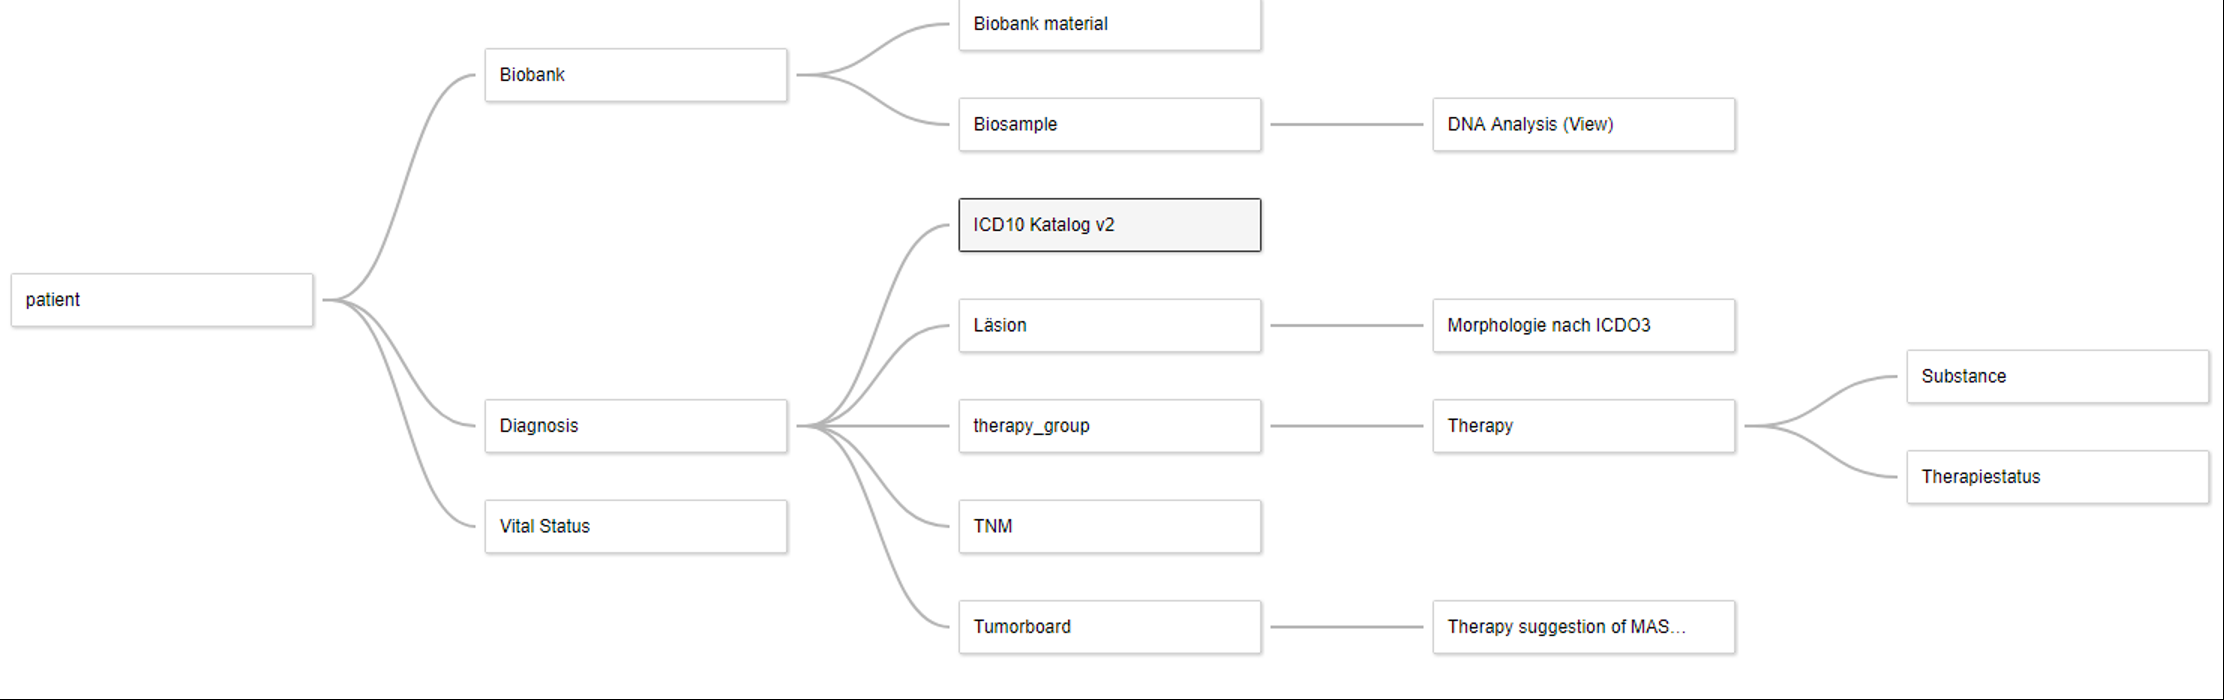
\includegraphics[width=0.7\textwidth]{images/datamodel_1.png}
\caption{Representation of the MIMIC Data Model: The squares represent CSV data tables the connections between the data tables represent the join relations used}\label{f1}
\end{figure}

\begin{table*}
\centering
\caption{Categories and their corresponding variables that the user can select to visualize}\label{t1}
\begin{tabular}{@{}ll@{}}
\hline
Category& Variables\\
\hline
Demographic information & age, ethnicity, gender, marital status, religion\\
Administrative information & admission ICU service type, admission source, admission type, number of days between ICU and hospital admissions, insurance type  \\
Patient outcomes & mortality at 28 days post-discharge from the hospital, hospital length of stay, hospital mortality, ICU mortality, ICU length of stay, 2-year survival days post-discharge from the hospital\\
Vital signs & heart rate, mean arterial blood pressure, oxygen saturation, respiratory rate, systolic blood pressure, body temperature \\
Lab test results & bicarbonate, calcium, chlorine, creatinine, glucose, hematocrit, lactate, magnesium, phosphorus, potassium, sodium, white blood cell count \\
Interventions & hemodialysis, peritoneal dialysis, total time on mechanical ventilation, vasopressor administration\\
Miscellaneous & amount of colloids administered, amount of crystalloids administered, body mass index, fluid balance, height, primary ICD-9, SOFA (sequential organ failure assessment) score, SAPS (simplified acute physiology score) I score, urine output, weight
\hline
\end{tabular}
\end{table*}